%compile with pdflatex on papeeria

\documentclass[a4paper,12pt]{article}


\usepackage{fontawesome}
\usepackage{fancyhdr}
\usepackage{fancyheadings}
\usepackage[ngerman,german]{babel}
\usepackage{german}
\usepackage[utf8]{inputenc}
%\usepackage[latin1]{inputenc}
\usepackage[active]{srcltx}
%\usepackage{svg}
%\usepackage{algorithm}
%\usepackage[noend]{algorithmic}
\usepackage{eurosym}
\usepackage{amsmath}
\usepackage{amssymb}
\usepackage{amsthm}
\usepackage{bbm}
\usepackage{enumerate}
\usepackage{graphicx}
\usepackage{ifthen}
\usepackage{listings}
\usepackage{enumitem}
%\usepackage{struktex}
\usepackage{hyperref}
\usepackage{tikz}
\usepackage{float}
\usepackage{subcaption}
\usepackage{array}
\captionsetup{compatibility=false}
\captionsetup[subfigure]{labelformat=empty}

\usepackage{pgfplots}
\pgfplotsset{compat=1.15}
\usepackage{mathrsfs}
\usetikzlibrary{arrows}

\definecolor{ccqqqq}{rgb}{0.8,0,0}
\definecolor{kolorwykresu}{rgb}{0.07,0.04,0.56}

\pagenumbering{gobble}

\usepackage{tabularray}
\usepackage{multirow}
\usepackage{booktabs,tabularx}

%\DeclareMathSymbol{\shortminus}{\mathbin}{AMSa}{"39}

\renewcommand\tabularxcolumn[1]{m{#1}}% for vertical centering text in X column

\newcolumntype{L}[1]{>{\raggedright\let\newline\\\arraybackslash\hspace{0pt}}m{#1}}
\newcolumntype{C}[1]{>{\centering\let\newline\\\arraybackslash\hspace{0pt}}m{#1}}
\newcolumntype{R}[1]{>{\raggedleft\let\newline\\\arraybackslash\hspace{0pt}}m{#1}}

\newcolumntype{Y}{>{\centering\arraybackslash}X}

%%%%%%%%%%%%%%%%%%%%%%%%%%%%%%%%%%%%%%%%%%%%%%%%%%%%%%
%%%%%%%%%%%%%% EDIT THIS PART %%%%%%%%%%%%%%%%%%%%%%%%
%%%%%%%%%%%%%%%%%%%%%%%%%%%%%%%%%%%%%%%%%%%%%%%%%%%%%%
\newcommand{\Fach}{2. Klausur aus der Mathematik}
\newcommand{\Name}{}
\newcommand{\datum}{}
\newcommand{\Matrikelnummer}{}
\newcommand{\Semester}{Q12/2}
\newcommand{\Uebungsblatt}{} %  <-- UPDATE ME
%%%%%%%%%%%%%%%%%%%%%%%%%%%%%%%%%%%%%%%%%%%%%%%%%%%%%%
%%%%%%%%%%%%%%%%%%%%%%%%%%%%%%%%%%%%%%%%%%%%%%%%%%%%%%

\setlength{\parindent}{0em}
\topmargin -1.0cm
\oddsidemargin 0cm
\evensidemargin 0cm
\setlength{\textheight}{9.2in}
\setlength{\textwidth}{6.0in}


\newcounter{aufgabencounter}
\newcommand{\aufgabeNr}{\stepcounter{aufgabencounter}{\theaufgabencounter}}

\newcommand{\Aufgabe}[1]{
  {
  \vspace*{0.5cm}
  \textsf{\textbf{Aufgabe \aufgabeNr #1}}
  \vspace*{0.2cm}
  
  }
}

%\newcommand{\Aufgabe}[1]{
%  {
%  \vspace*{0.5cm}
%  \textsf{\textbf{Aufgabe #1}}
%  \vspace*{0.2cm}
%  
%  }
%}
%%%%%%%%%%%%%%
\hypersetup{
    pdftitle={\Fach{}: Übungsblatt \Uebungsblatt{}},
    pdfauthor={\Name},
    pdfborder={0 0 0}
}

\lstset{ %
language=java,
basicstyle=\footnotesize\tt,
showtabs=false,
tabsize=2,
captionpos=b,
breaklines=true,
extendedchars=true,
showstringspaces=false,
flexiblecolumns=true,
}

\newcommand*{\quadratbox}{\textbf{\fbox{\phantom{\huge{?}}}}}%

\title{Übungsblatt \Uebungsblatt{}}
\author{\Name{}}

\begin{document}

\fancyhead{}
\fancyhead[C]{\includegraphics[height=2.5cm]{lukasLogoV2.png}
\vspace{2cm}
}

\thispagestyle{fancy}

\lhead{
%\vspace{1cm}
  \sf \LARGE \Fach{} %\small \Name{} - \Matrikelnummer{}
}
\rhead{\sf \Semester{}   \datum{}}


\vspace*{0.2cm}

\vspace{4cm}
Alle Lösungen müssen mit Nebenrechnungen und Begründungen nachvollziehbar sein!

%\rhead{\sf \Semester{} }
\vspace*{0.2cm}

%\begin{center}
%%\LARGE \sf \textbf{Übungsblatt \Uebungsblatt{}}
%\end{center}
%\vspace*{0.2cm}

%%%%%%%%%%%%%%%%%%%%%%%%%%%%%%%%%%%%%%%%%%%%%%%%%%%%%%
%% Insert your solutions here %%%%%%%%%%%%%%%%%%%%%%%%
%%%%%%%%%%%%%%%%%%%%%%%%%%%%%%%%%%%%%%%%%%%%%%%%%%%%%%

\vspace{1cm}
  Name: \underline{\hspace{7cm}}
  \hfill
  Datum: \underline{\hspace{4cm}}

\vspace{0.8cm}

%\textbf{Hinweise:} Der Lösungsweg muss nachvollziehbar sein. Arbeitszeit \textbf{45 Minuten}.
%\vspace{0,5cm}Die Rechenwege müssen nachvollziehbar sein!
%
%\vspace{0,5cm} {TEIL A} - ohne Hilfsmittel - Bearbeitungszeit 30 Minuten
%\vspace {0.8cm}
% 
%GEOMETRIE


\begin{center}
  \begin{tblr}{
      width=1\linewidth,
      colspec = {Q[c,6em]Q[c,3em]Q[c,3em]Q[c,3em]Q[c,3em]Q[c,3em]Q[c,3em]Q[c,3em]Q[c,6em]Q[c,6em]},
      rowspec = {Q[m]Q[m]Q[m]Q[m]Q[m]Q[m]Q[m]Q[m]Q[m]Q[m]},
      colsep = 0mm,
      %row{1} = {2em,azure2,fg=white,font=\large\bfseries\sffamily},
      row{1} = {2em,font=\large\bfseries\sffamily},
      hlines, vlines,
    }
    \textbf{Aufgabe} & \textbf{1} & \textbf{2} & \textbf{3} & 
    \textbf{4} & \textbf{5} & \textbf{6}& \textbf{7}& \textbf{Gesamt} & \textbf{Note}\\
    {Mögliche \\ Punkte} &5 &4 &5 &15 &5 &14 &8 & 56  \\
    {Erreichte \\ Punkte} &  &  &  &  & & & & & \\
  \end{tblr}
\end{center}

\vspace{0.3cm}
%\newpage\null\thispagestyle{empty}\newpage
\newpage
\vspace{1,5cm} {TEIL A} - ohne Hilfsmittel.
\vspace {0,2cm}

\Aufgabe{: (5BE)}
  Die folgende Darstellung zeigt den Graphen einer Funktion $f$.

  \begin{figure}[H]
    \vspace{0cm}
    \centering
    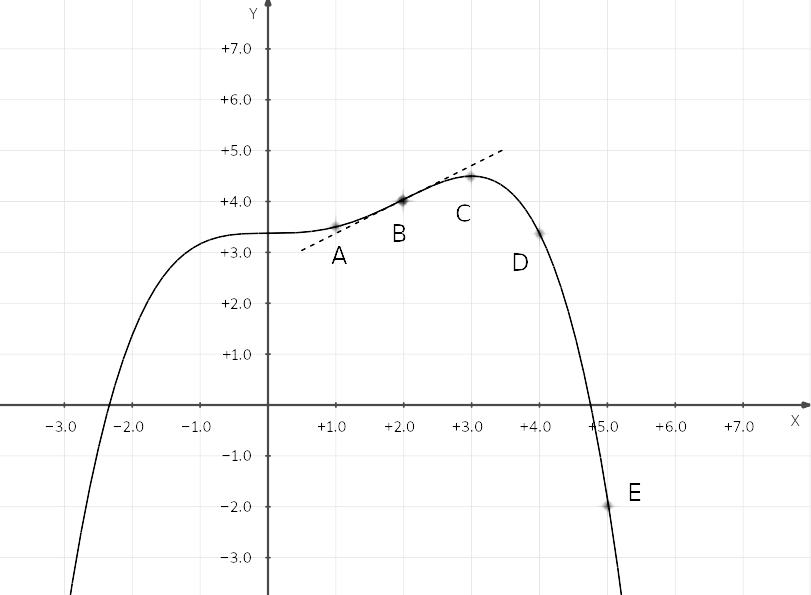
\includegraphics[width=0.9\linewidth]{Klausur_240215_1.jpg}
  \end{figure}

Geben Sie für die Punkte $A$ bis $E$ an, ob die Werte von $f$, $f'$ (1. Ableitungsfunktion) und $f''$ (2. Ableitungsfunktion) jeweils positiv, negativ oder null ist.


\begin{center}
  \begin{tblr}{
      width=1\linewidth,
      colspec = {Q[c,6em]Q[c,6em]Q[c,6em]Q[c,6em]},
      rowspec = {Q[m]Q[m]Q[m]Q[m]},
      colsep = 0mm,
      %row{1} = {2em,azure2,fg=white,font=\large\bfseries\sffamily},
      row{1} = {2em,font=\large\bfseries\sffamily},
      hlines, vlines,
    }
      & \textbf{$f$} & \textbf{$f'$} & \textbf{$f''$} \\
    \textbf{A} &  &  &  \\
    \textbf{B} &  &  &  \\
    \textbf{C} &  &  &  \\
    \textbf{D} &  &  &  \\
    \textbf{E} &  &  &  \\
  \end{tblr}
\end{center}

\Aufgabe{: (4BE)}
Begründen Sie rechnerisch: Eine Funktion 2ten Grades $f: x \rightarrow ax^2 + bx + c$ mit $a\neq 0$ besitzt keinen Wendepunkt. Geben Sie weiter das Krümmungsverhalten in Abhängigkeit von $a$ an.
\newpage

\Aufgabe{: (5BE)}
Im folgenden Koordinatensystem ist der Graph der punktsymmetrischen Funktion $g$ dargestellt.

  \begin{figure}[H]
    \vspace{0cm}
    \centering
    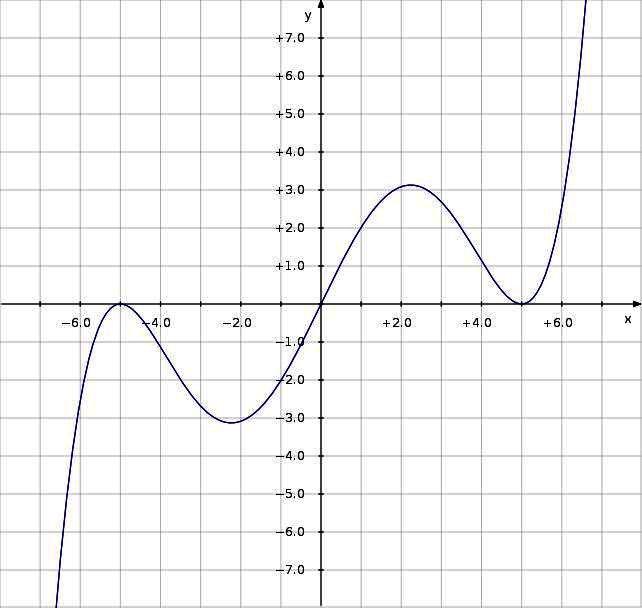
\includegraphics[width=1\linewidth]{Klausur_240215_2.jpg}
  \end{figure}

  $A$ ist die Fläche zwischen der $x$-Achse und dem Graphen der Funktion $g$.
  \begin{enumerate}[label={(\alph*)}]
    \item $G$ ist Stammfunktion von $g$. Ermitteln Sie mit Hilfe der beiden Werte $G(0)=-2$ und $G(5)=7$, den Inhalt der genannten Fläche $A$.
    \item Gib $G(-5)$ an.
  \end{enumerate}

%\newpage
%\vspace*{-2cm}
\newpage
\vspace{1,5cm} {TEIL B} - mit Hilfsmitteln.
\vspace {0,2cm}

\Aufgabe{: (2+3+3+5+2=15BE)}
Die Fluggesellschaft Comfortflights bietet bei Mittel- und Langstreckenflügen Decken für fröstelnde Fahrgäste an. Aus Platzgründen kann nicht für jeden Fahrgast eine Decke zur Verfügung gestellt werden. Da für Unternehmensleitung die Kundenzufriedenheit eine hohe Priorität hat, möchte Sie für verschiedene Situationen die Wahrscheinlichkeit wissen. Aus Erfahrung weiß man, dass sich im Mittel 15\% der Passagiere für eine Decke entscheiden. Im Folgenden soll davon ausgegangen werden, dass die Passagiere sich unabhängig voneinander für eine Decke entscheiden bzw. dagegen.
\begin{enumerate}[label={\alph*)}]
  \item Bestimmen Sie mit welcher Wahrscheinlichkeit sich genau 20 von 100 Passagieren eine Decke wünschen?
  \item Berechnen Sie mit welcher Wahrscheinlichkeit sich mindestens 20 von 100 Passagieren  eine Decke wünschen?
  \item Die Passagiere steigen der Reihe nach ins Flugzeug. Berechnen Sie mit welcher Wahrscheinlichkeit der 20. Passagier derjenige ist, der sich die 3. Decke wünscht.
  \item Berechnen Sie wie viele Passagieren mindestens an Bord sein müssen, damit sich mit einer Wahrscheinlichkeit von mindestens 99\% mindestens ein Passagier eine Decke wünscht?
  \item Geben Sie der Unternehmensleitung eine Empfehlung, wie viele Decken sie bei einem Passagierflugzeug mit 100 Plätzen mitnehmen soll. Begründen Sie Ihre Empfehlung u.a. mit Werten aus dem Tafelwerk.
\end{enumerate}

\Aufgabe{: (5BE)}
Zur Montage eines Gerätes benötigt eine Firma ein Verbindungsstück $V$, das nicht im eigenen Betrieb hergestellt wird. Der Hersteller von $V$ behauptet, dass der Ausschussanteil höchstens 10\% beträgt. Der Hersteller von $V$ bietet an, dass man eine Lieferung zurückweisen darf, wenn in einer Stichprobe von 100 Bauteilen mehr als $k$ defekt sind. Für welchen Wert von $k$ kann man mit mindestens 95\% Sicherheit die Behauptung des Herstellers zurückweisen?

\newpage
\Aufgabe{: (4+4+4+2=14BE)}
Gegeben sind die Punkte $A(1|-2|2)$, $B(4|3|0)$, $C(0|-7|7)$ und $D(-4|-7|1)$. 
\begin{enumerate}[label={\alph*)}]
  \item Zeigen Sie, dass die vier Punkte in einer Ebene $E$ liegen!
  \item Geben Sie eine Gleichung dieser Ebene in Parameter- und in Koordinatenform an!

    \[\text{Ersatzergebnis:} E: \vec{X} = \begin{pmatrix} 2 \\ -2 \\ -1 \end{pmatrix} \;
      + \lambda \begin{pmatrix} 5 \\ -2 \\ 3 \end{pmatrix} \;
      + \mu \begin{pmatrix} 5 \\ -5 \\ 1 \end{pmatrix} \;
    \]
    \item Bestimmen Sie die Spurgerade der Ebene $E$ mit der $x_1x_3$-Ebene.
    \item Bestimmen Sie den Wert für $a$ so, dass die Gerade $h: \vec{X} = \begin{pmatrix} -8 \\ 9 \\ 10 \end{pmatrix} + \lambda \begin{pmatrix} a \\ 0 \\ 3 \end{pmatrix}$ parallel zur Ebene $E$ verläuft!
\end{enumerate}

\Aufgabe{: (2+4+2=8BE)}
Sie sind Praktikant in einem Architekturbüro und sollen überprüfen, ob ein von einer Lichtquelle $L(0|6|15)$ in Richtung $\vec{r} = \begin{pmatrix} 2 \\ -1 \\ -3 \end{pmatrix}$ ausgehender Lichtstrahl den Stab $[AB]$ mit den Endpunkten $A(1|-5|6)$ und $B(3|1|8)$ trifft. 
\begin{enumerate}[label={\alph*)}]
\item Stellen Sie die Gleichungen der Geraden $h$ des Lichtstrahls und der Gerade $AB$ auf.
\item Untersuchen Sie die Lagebeziehung der Geraden $h$ und $AB$.
\item Geben Sie Ihrem Architekten eine Antwort mit stichhaltiger Begründung auf die Ihnen gestellte Aufgabe.
\end{enumerate}

\vspace{2cm}
\centerline{Viel Erfolg \faThumbsOUp }

\newpage
{
\Huge{MUSTERLÖSUNG}
}

\small

\textbf{Aufgabe 1}
\begin{center}
  \begin{tblr}{
      width=1\linewidth,
      colspec = {Q[c,6em]Q[c,6em]Q[c,6em]Q[c,6em]},
      rowspec = {Q[m]Q[m]Q[m]Q[m]},
      colsep = 0mm,
      %row{1} = {2em,azure2,fg=white,font=\large\bfseries\sffamily},
      row{1} = {2em,font=\large\bfseries\sffamily},
      hlines, vlines,
    }
      & \textbf{$f$} & \textbf{$f'$} & \textbf{$f''$} \\
    \textbf{A} & + & + & + \\
    \textbf{B} & + & + & o \\
    \textbf{C} & + & o & - \\
    \textbf{D} & + & - & - \\
    \textbf{E} & - & - & - \\
  \end{tblr}
\end{center}

  \begin{figure}[H]
    \vspace{0cm}
    \centering
    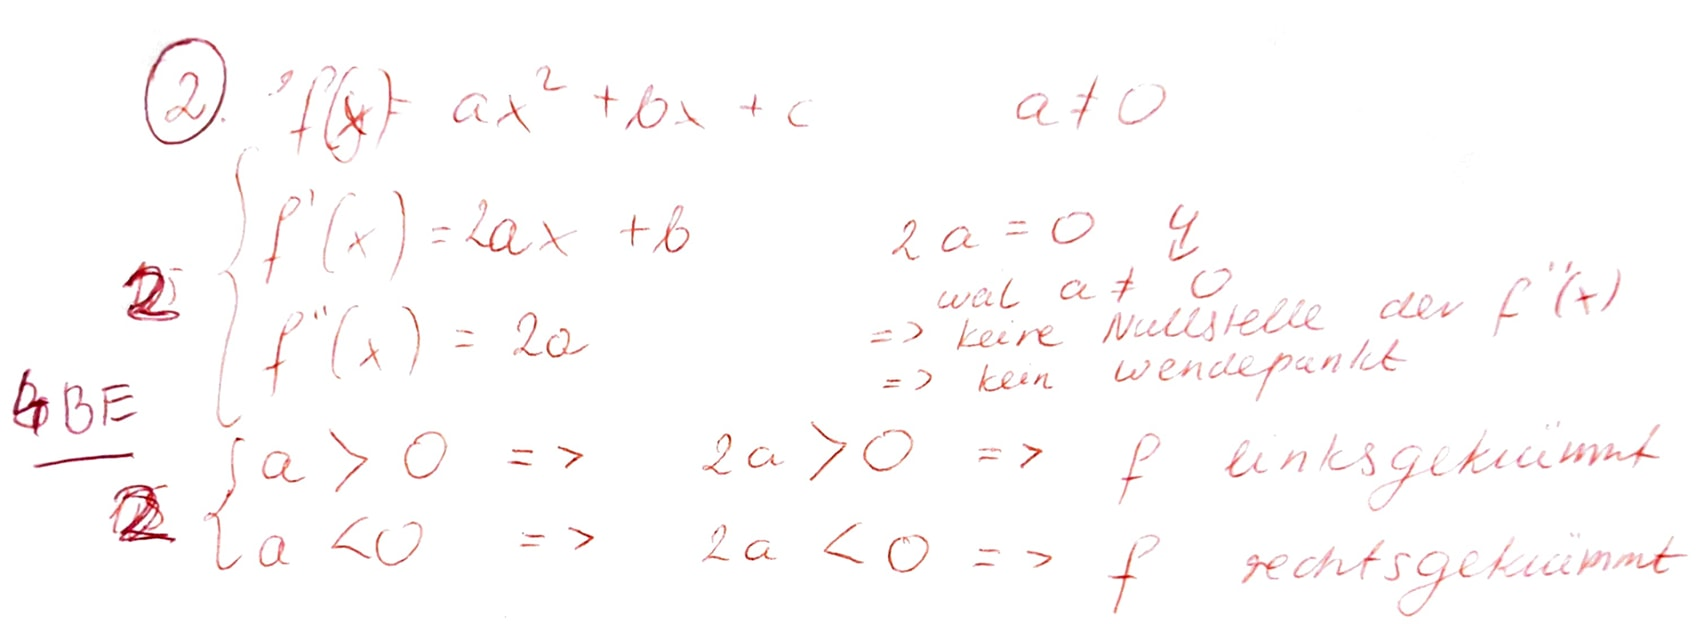
\includegraphics[width=1\linewidth]{ml_240215_A2.jpg}
  \end{figure}

  \begin{figure}[H]
    \vspace{0cm}
    \centering
    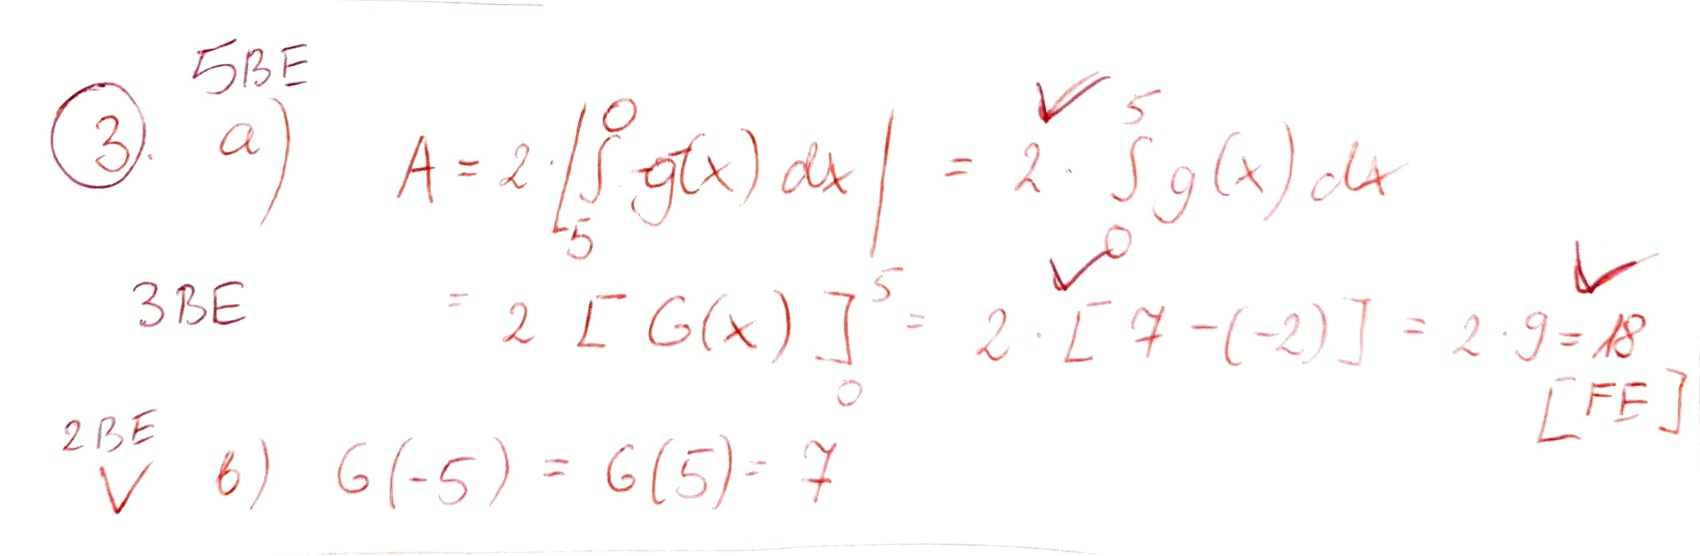
\includegraphics[width=1\linewidth]{ml_240215_A3.jpg}
  \end{figure}



  \begin{figure}[H]
    \vspace{0cm}
    \centering
    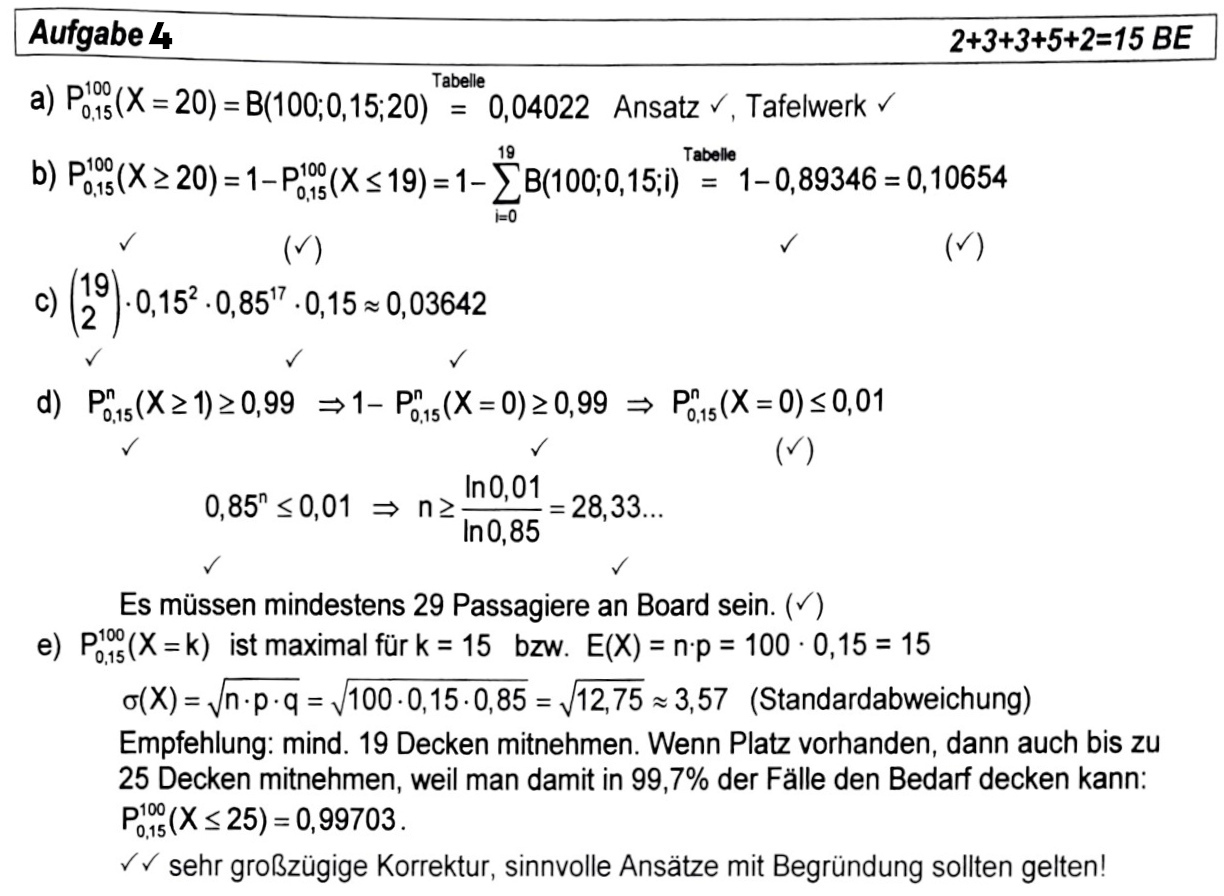
\includegraphics[width=1\linewidth]{ml_240215_1a.jpg}
  \end{figure}

  Aufgabe 5
  \begin{figure}[H]
    \vspace{0cm}
    \centering
    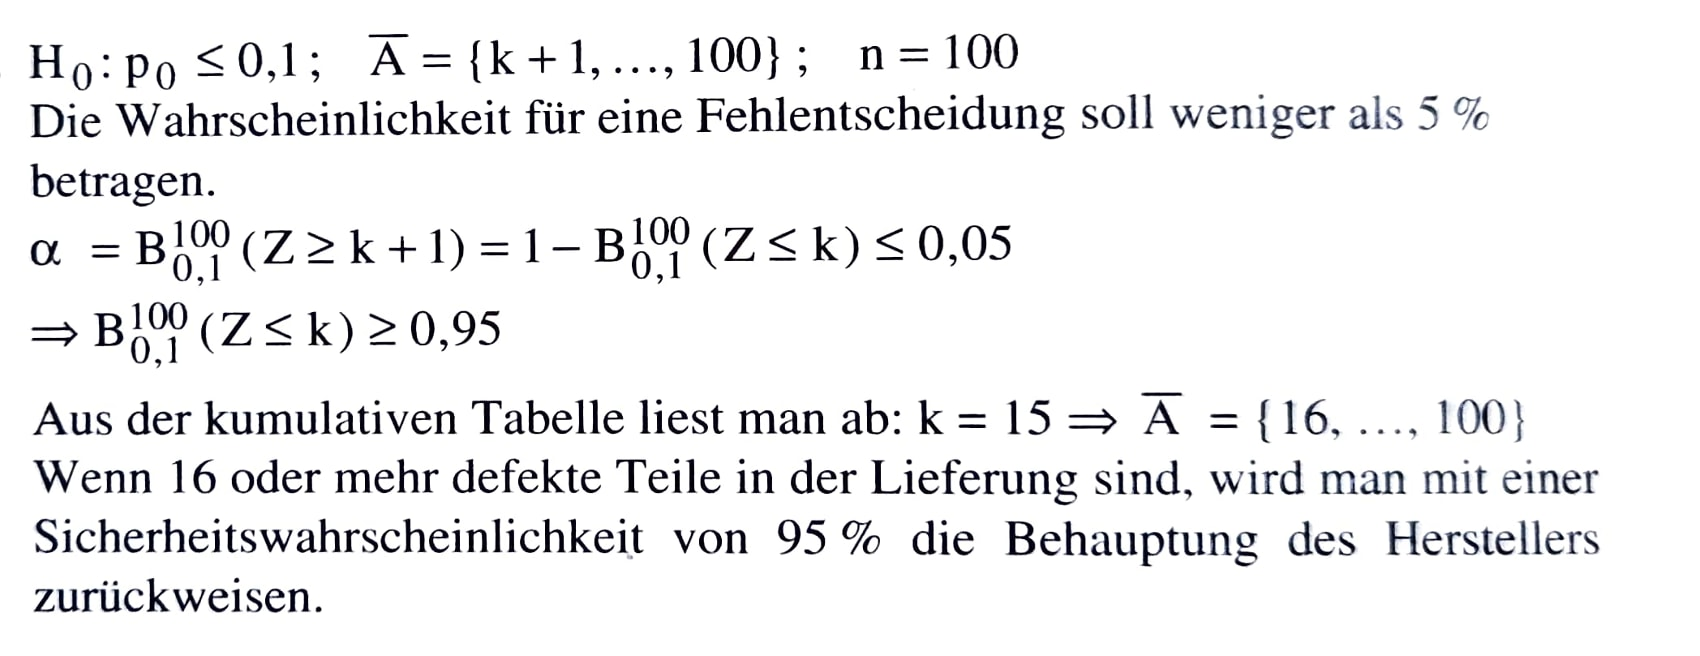
\includegraphics[width=1\linewidth]{ml_240215_new2.jpg}
  \end{figure}


  Aufgabe 6 und 7
  \begin{figure}[H]
    \vspace{0cm}
    \centering
    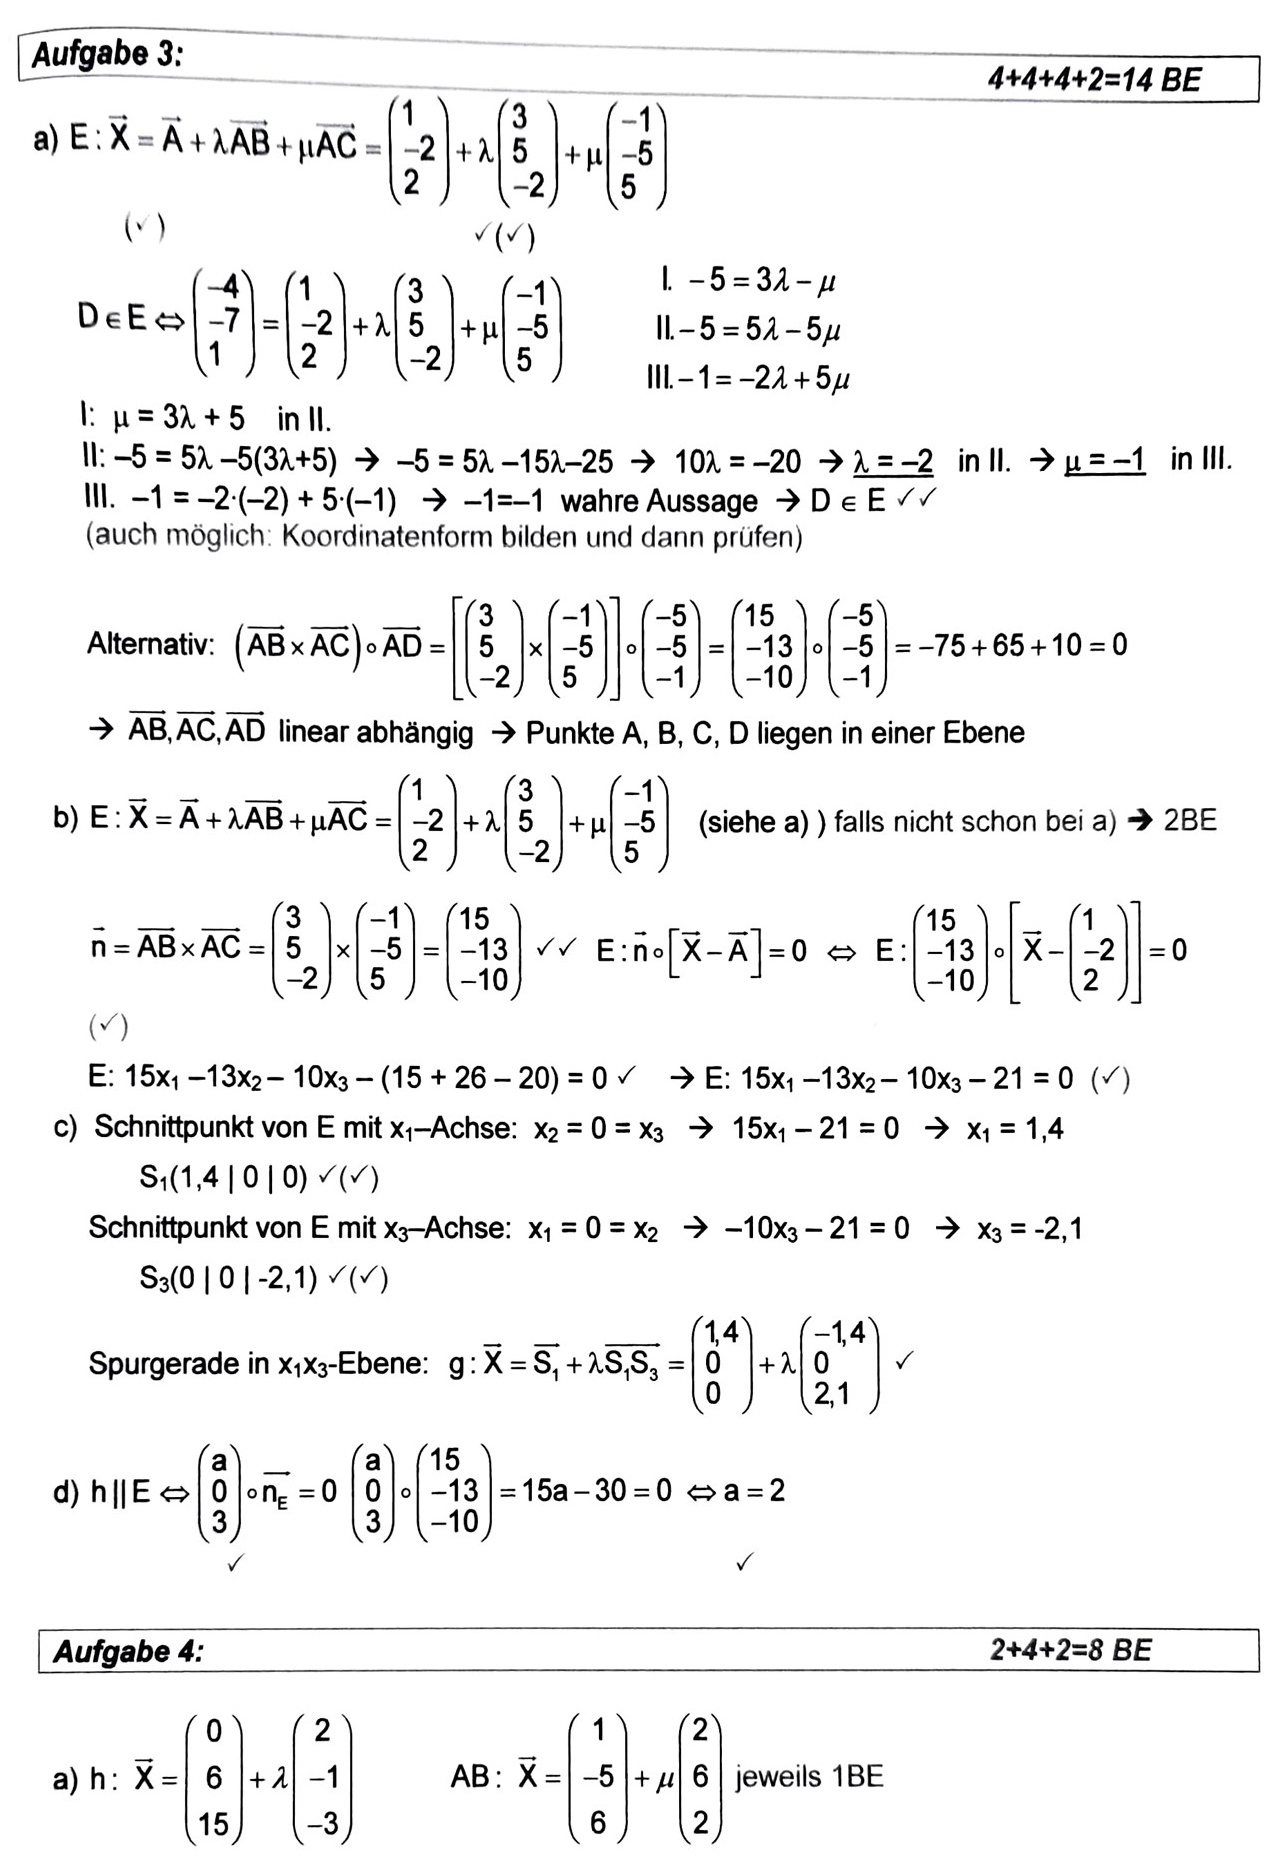
\includegraphics[width=0.9\linewidth]{ml_240215_2.jpg}
  \end{figure}

  \begin{figure}[H]
    \vspace{0cm}
    \centering
    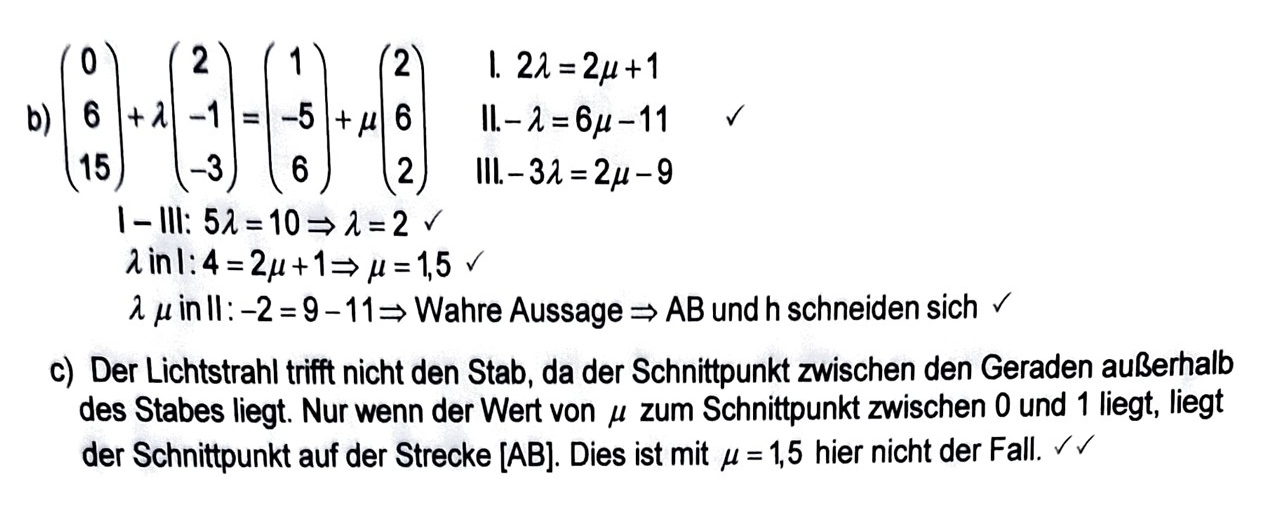
\includegraphics[width=0.9\linewidth]{ml_240215_3.jpg}
  \end{figure}

\Aufgabe{: NACHSCHREIBEN (3+3+2=8BE)}
Bei einer Schulfahrt mit 10 Schülern und 2 Lehrern sind für die Reisegruppe 12 Plätze für einen Flug nach Sibirien gebucht. Da im Mittel 5\% der Buchungen storniert werden, verkauft die Fluggesellschaft 200 Tickets, obwohl für den Flug nur 190 Plätze zur Verfügung stehen.
\begin{enumerate}[label={\alph*)}]
  \item Bestimmen Sie die Wahrscheinlichkeit für den Fall, dass die Plätze nicht ausreichen.
  \item Berechnen Sie die Wahrscheinlichkeit dafür, dass mehr als 3 Platze frei bleiben.
  \item Beim Abflug stellt sich heraus, dass fünf Fluggäste zu viel am Gate erscheinen. Es werden nun die fünf Fluggäste ausgelost, die nicht mitfliegen können. Berechnen Sie wie groß die Wahrscheinlichkeit dafür ist, dass genau ein Lehrer und genau ein Schüler nicht mitfliegen dürfen.
\end{enumerate}

  \begin{figure}[H]
    \vspace{0cm}
    \centering
    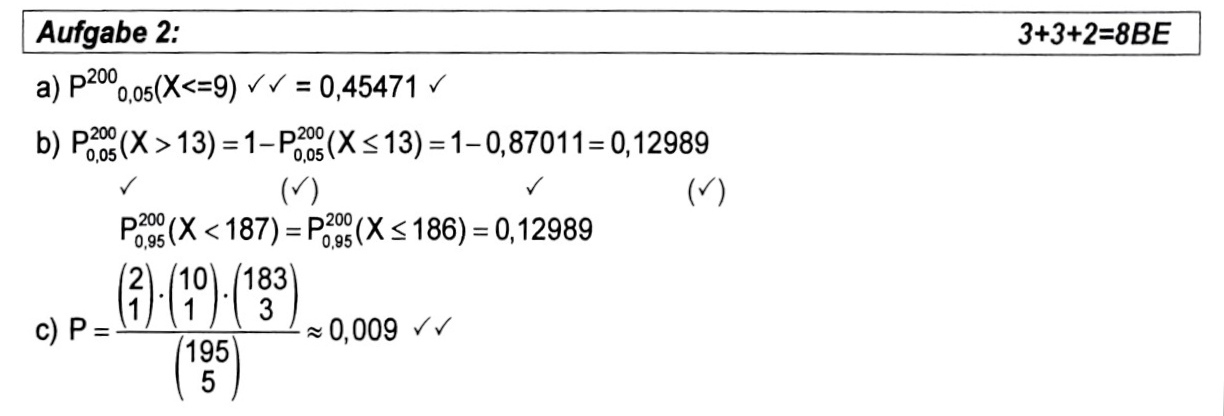
\includegraphics[width=1\linewidth]{ml_240215_2a.jpg}
  \end{figure}

\end{document}
